\documentclass[margin=0.1in]{standalone}
\usepackage{tikz}
\usepackage{stanli}
\begin{document}

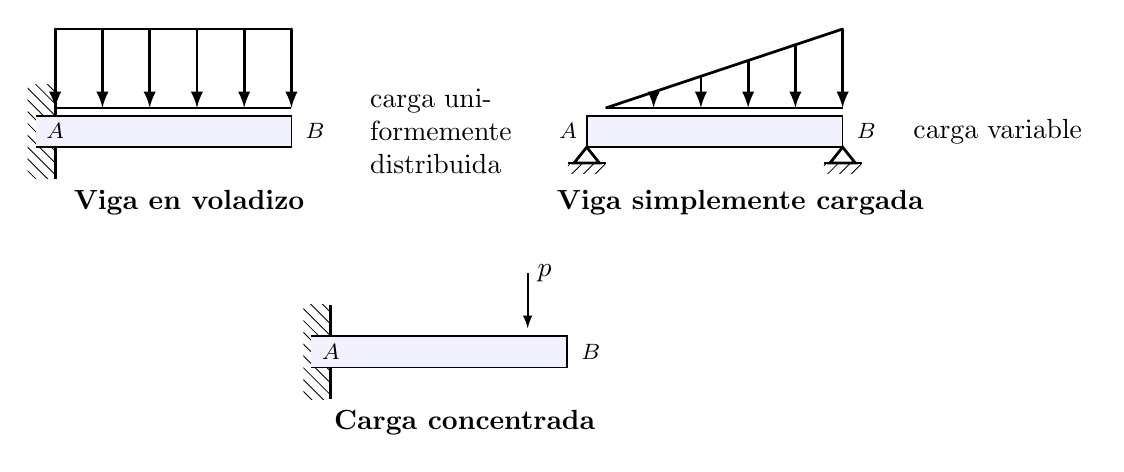
\begin{tikzpicture}[>=latex]
	% \clip (-0.5,0.2) rectangle ++(1,0.5) (-0.5,-0.2) rectangle ++(1,-0.5);
	\point{a}{0}{0};
	\support{3}{a}[-90];
	\fill [blue!5] (-0.25,-0.2) rectangle (3,0.2);
	\draw [semithick] (-0.25,-0.2) -- (3,-0.2) -- (3,0.2) -- (-0.25,0.2);
	\node at (a) {\footnotesize \(A\)};
	\node at (3.3,0) {\footnotesize \(B\)};
	\point{b}{3}{0}
	\lineload{1}{a}{b};
	\node [text width = 2cm] at (5,0) {carga uniformemente distribuida};
	\node at (1.7,-0.9) {\textbf{Viga en voladizo}};
	\begin{scope}[xshift=7cm]
		\point{a}{0}{0};
		\filldraw [fill=blue!5, semithick] (-0.25,-0.2) rectangle (3,0.2);
		\node [left] at (-0.25,0) {\footnotesize \(A\)};
		\node at (3.3,0) {\footnotesize \(B\)};
		\point{b}{3}{0};
		\lineload{1}{a}{b}[0];
		\begin{scope}[scale=0.4]
			\point{a}{-0.25}{-0.2};
			\point{b}{3}{-0.2};
			\support{1}{a};
			\support{1}{b};
		\end{scope}
		\node [text width = 2.2cm] at (5,0) {carga variable};
		\node at (1.7,-0.9) {\textbf{Viga simplemente cargada}};
	\end{scope}
	\begin{scope}[xshift=3.5cm, yshift=-2.8cm]
		\point{a}{0}{0};
		\support{3}{a}[-90];
		\fill [blue!5] (-0.25,-0.2) rectangle (3,0.2);
		\draw [semithick] (-0.25,-0.2) -- (3,-0.2) -- (3,0.2) -- (-0.25,0.2);
		\node at (a) {\footnotesize \(A\)};
		\node at (3.3,0) {\footnotesize \(B\)};
		\draw [semithick,->] (2.5,1) node [right] {\(p\)} --++ (0,-0.7);
		\node at (1.7,-0.9) {\textbf{Carga concentrada}};
	\end{scope}
\end{tikzpicture}

\end{document}
